\documentclass[
  11pt,
  letterpaper,
   addpoints,
  % answers
  ]{exam}

\usepackage{../exercise-preamble}
\usepackage{multicol}
\begin{document}

\noindent
\begin{minipage}{0.47\textwidth}

\includegraphics[width=\textwidth]{../fcfm_die}
\end{minipage}
\begin{minipage}{0.53\textwidth}
    
\begin{center} 
\large\textbf{Análisis y Diseño de Circuitos Eléctricos} (EL3101-2) \\
\large\textbf{Tarea 2} \\
\normalsize Prof.~Santiago Bradford V.\\
\normalsize Prof.~Aux.~Erik Saez A. - Rodrigo Catalán\\
             - Byron Castro R.
\end{center}
\end{minipage}

\vspace{0.5cm}
\noindent
\vspace{.85cm}

\fbox{%
  \begin{minipage}{0.95\linewidth}
    \textbf{Obs:} Recuerde que solo serán revisadas tres preguntas al azar. No olvide explicar de forma clara y precisa su desarrollo. \\\\
    \textbf{Fecha de entrega}: Domingo 1 de Junio
  \end{minipage}
}

\begin{questions}
    %%%%%%%%%%%%%%%%%%%%%%%%%%%%
    \question     
    \begin{enumerate}
    \item El \textit{switch} del circuito de la figura 1 ha estado cerrado por un largo periodo de tiempo. En $t=0$, este cambia su posición abriéndose.
    \begin{enumerate}
        \item Calcular la corriente y caídas de tensión instantáneas en $R$, $L$ y $C$ en régimen transitorio.
        \item Esbozar un gráfico de la corriente por la rama $RLC$ del circuito (parte derecha), indicando el tipo de amortiguamiento presente.
        \item Calcular la carga acumulada y energía almacenada en el condensador $C$ en régimen permanente.
    \end{enumerate}
        \begin{center}
            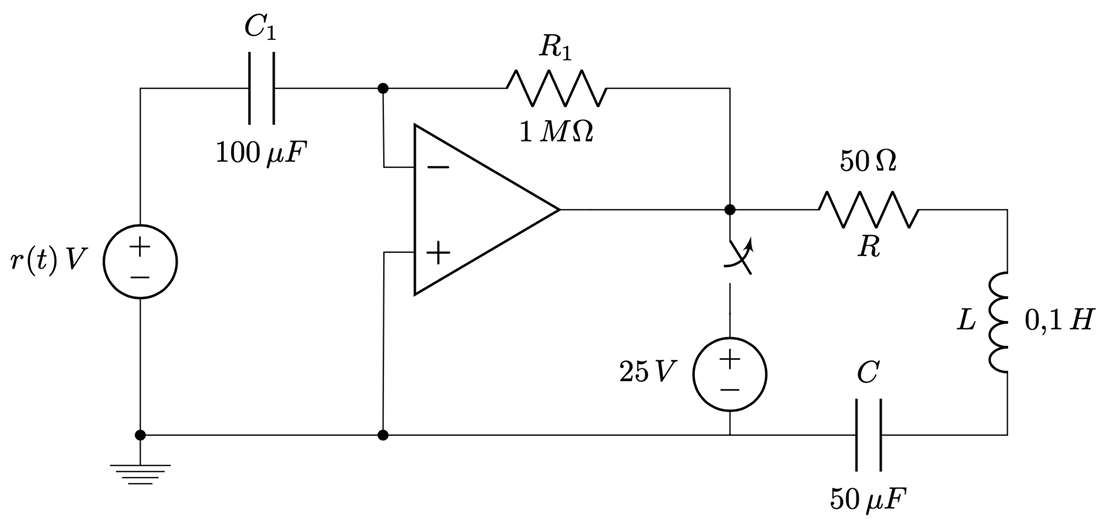
\includegraphics[width=0.6\textwidth]{Tarea_2_1}
            \captionof{figure}{Esquema del problema}
        \end{center}
    \end{enumerate}
    %%%%%%%%%%%%%%%%%%%%%%%%%%%%
    \begin{solution}
        a
    \end{solution}
    %%%%%%%%%%%%%%%%%%%%%%%%%%%
    \question   El circuito de la figura 2 ha estado en la posición $A$ por un largo periodo de tiempo. Este pasa a la posición $B$ en $t=0[s]$, para volver nuevamente a la posición $A$ en $t=50[\mu s]$. Calcule $v_c(t)$ para $t\geq 0$, separando la respuesta a entrada cero y respuesta de estado cero en cada intervalo de tiempo que usted defina.

    \begin{center}
        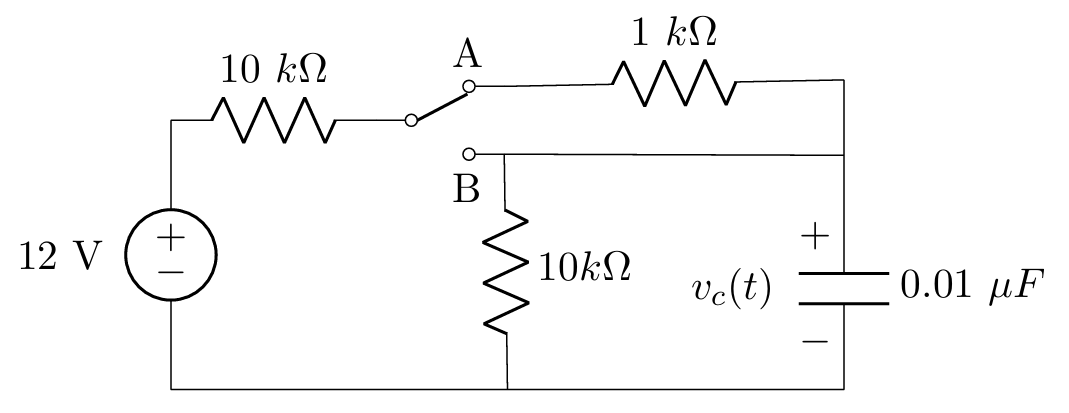
\includegraphics[width=0.6\textwidth]{Tarea_2_2}
        \captionof{figure}{Esquema del circuito}
    \end{center}
    %%%%%%%%%%%%%%%%%%%%%%%%%%%
    \begin{solution}
       a
    \end{solution}
%%%%%%%%%%%%%%%%%%%%%%%%%%%
\question Usando el método de convolución gráfica, determine el resultado de la convolución entre las siguientes configuraciones de respuesta al impulso $h(t)$ y entrada $i(t)$. Para cada caso, especifique los intervalos y límites de integración, junto con una gráfica del resultado.
\begin{center}
    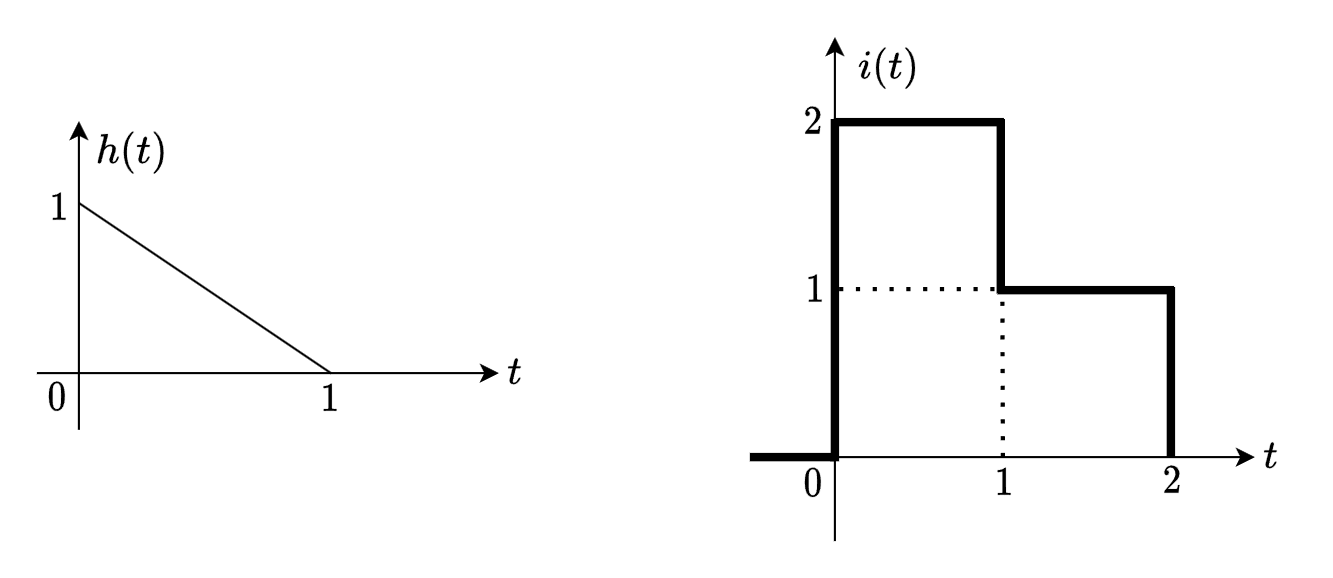
\includegraphics[width=0.45\textwidth]{Tarea_2_3}
    \captionof{figure}{Esquema del circuito}
\end{center}
\begin{center}
    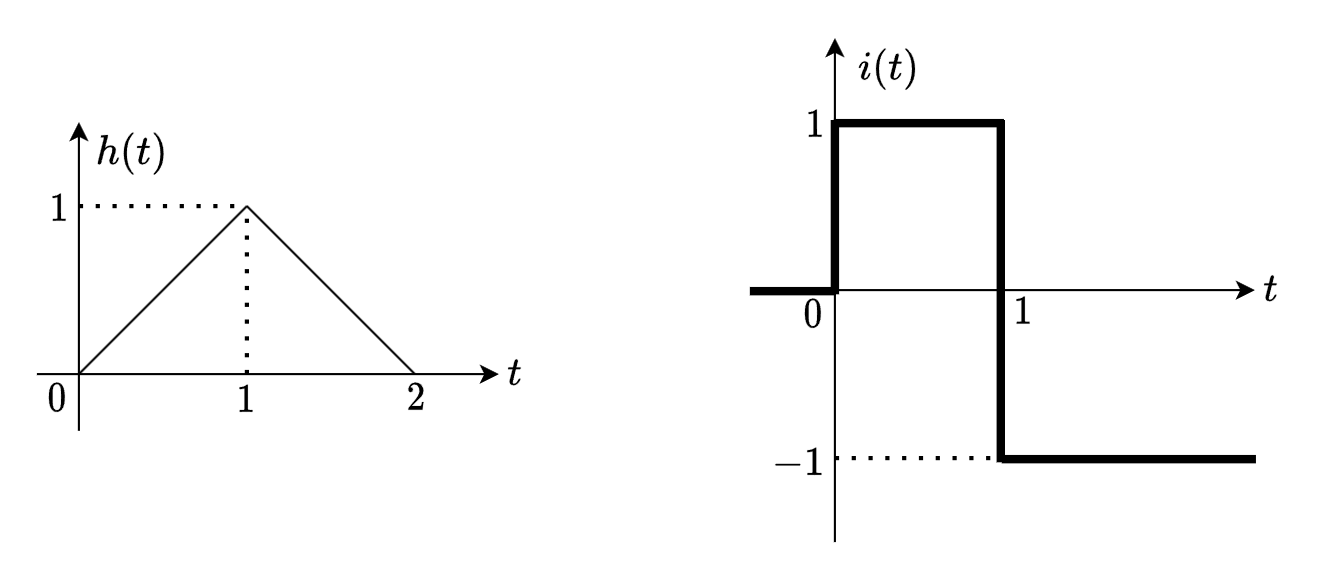
\includegraphics[width=0.45\textwidth]{Tarea_2_4}
    \captionof{figure}{Esquema del circuito}
\end{center}
%%%%%%%%%%%%%%%%%%%%%%%%%%%
\begin{solution}
    a
\end{solution}
%%%%%%%%%%%%%%%%%%%%%%%%%%%
\question Durante una de las exploraciones de un astronauta, el resorte de su vehículo se dañó quedando a la deriva y sin comunicación con el centro de mando. El Astronauta recuerda de su entrenamiento, la masa \( m \) del vehículo, la constante de amortiguamiento \( c \) y la longitud de onda promedio de la superficie lunar \( L \) de la zona donde se encuentra Además puede desoldar los Opamps, resistencias y condensadores de su propio vehículo. Ante ello, usted debe ayudar al astronauta a construir una computadora analógica capaz de resolver la ecuación diferencial que modela el movimiento de su vehículo. Luego, la idea es que establezca un criterio para decidir qué resorte de repuesto \( k \) puede reducir lo máximo posible las oscilaciones del vehículo dado que el suelo lunar se puede modelar por \( y(t) = a \cos \left( \frac{2 \pi s(t)}{L} \right) \) donde \( s(t) \) es la distancia recorrida por el vehículo. Para ello considere que la ecuación diferencial que modela el movimiento del vehículo es:

\begin{equation}
\ddot{x}(t) + \frac{c}{m} \dot{x}(t) + \frac{k}{m} x(t) = \frac{ka}{m} \cos \left( \frac{2 \pi v t}{L} \right)
\quad \text{con} \quad x(0) = l_0 + a, \quad \dot{x}(0) = 0
\end{equation}

\begin{enumerate}
    \item Diseñar un circuito con solo tres Opamps, seis resistencias, dos condensadores y dos fuentes de voltaje. Recuerde plasmar en su circuito las condiciones iniciales. Encuentre además las relaciones de las resistencias y capacitores respecto a las constantes de la ecuación diferencial.
    
    \item Exprese la raíz del polinomio característico de la ecuación diferencial planteada en el ítem anterior. Identifique a \( \alpha \) y \( w_0 \) en \( \lambda = -\alpha \pm \sqrt{\alpha^2 - w_0^2} \).
    
    \item El astronauta prefiere que el vehículo esté lo más estable posible a corto plazo, ante ello, de la pregunta anterior establezca qué condición deba cumplir el resorte \( k \) para que esto suceda. Apoye su respuesta con un análisis breve y cualitativo del tiempo en que tarda \( x(t) \) en estabilizarse según la restricción de \( k \).
\end{enumerate}
\begin{center}
    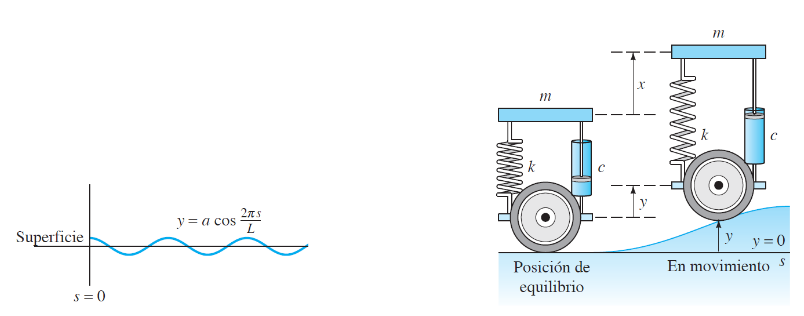
\includegraphics[width=0.7\textwidth]{Tarea_2_5}
    \captionof{figure}{Esquema del circuito}
\end{center}
%%%%%%%%%%%%%%%%%%%%%%%%%%%%%
\question Para el circuito de la figura 6 determine \( v_0(t) \) para \( t > 0 \) cuando \( R = 100 \, \text{k}\Omega \) y \( C = 1 \, \mu\text{F} \).

Considere además que \( v_1(0^+) = 2 \, \text{V} \) y \( v_2(0^+) = 0 \, \text{V} \).

\begin{center}
    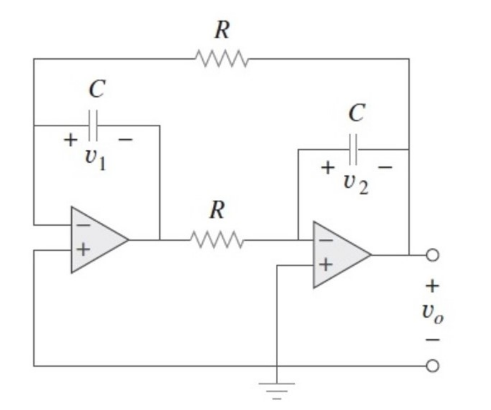
\includegraphics[width=0.45\textwidth]{Tarea_2_6}
    \captionof{figure}{Esquema del circuito}
\end{center}
%%%%%%%%%%%%%%%%%%%%%%%%%%%
\begin{solution}
   A
\end{solution}
%%%%%%%%%%%%%%%%%%%%%%%%%%%

\question En el circuito de la Figura 2, los switches operan sincrónicamente: cuando el switch de la izquierda está en la posición A, el switch de la derecha está en la posición D; cuando el switch de la izquierda está en la posición B, el switch de la derecha está en la posición C.

En \( t = 0 \), los switches se mueven a su posición final. Determine \( v_o(t) \) para \( t \geq 0 \), suponiendo que los switches han estado en su posición inicial durante mucho tiempo.

\begin{center}
    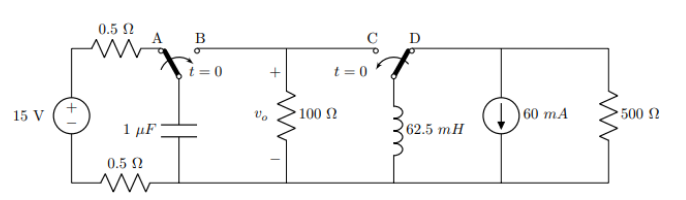
\includegraphics[width=0.7\textwidth]{Tarea_2_7}
    \captionof{figure}{Esquema del circuito}
\end{center}
\end{questions}
\end{document}